\appendix

\phantomsection
\section*{Appendix}


\begin{itemize}
  \item[] \textbf{\ref{app:benchmarks} Benchmark Construction and Implementation Details}
    \begin{itemize}
      \item[] \ref{app:fir_extraction} Extraction of Functional Intermediate Representations
      \item[] \ref{app:mppi_annotation} MPPI-based Demonstration Generation
      \item[] \ref{app:implementation_details} Training and Implementation Details
    \end{itemize}
    
  \item[] \textbf{\ref{app:additional_experimental_results} Additional Experimental Results}
    \begin{itemize}
      % \item[] \ref{app:more_real_world_experiments} More Real-World Experiments
      % \item[] \ref{app:more_qualitative_results} Additional Qualitative Comparisons
      \item[] \ref{app:more_qualitative_results_real} More Qualitative Results in the Real World
      \item[] \ref{app:more_qualitative_results_sim} More Qualitative Results in Simulation
      % \item[] \ref{app:visual_robustness} Additional Qualitative Comparisons in the Real World
    \end{itemize}
\end{itemize}



\section{Benchmark Construction and Implementation Details}
\label{app:benchmarks}

This section provides additional details on benchmark construction and implementation.
We first describe the extraction of different functional intermediate representations in Appx.~\ref{app:fir_extraction}, including those used for representation selection and human-video pretraining.
We then introduce our MPPI-based demonstration generation procedure in Appx.~\ref{app:mppi_annotation}, using the hitting function as a representative example.
Finally, we summarize the training and implementation details of \algoname{} and all baselines in Appx.~\ref{app:implementation_details}.

\begin{table}[ht]
\centering
\caption{\textbf{Statistics of Functional Intermediate Representations for Hitting.}
We report the number of tools, settings, initial configurations, samples per configuration, and total samples used for each representation.}
\label{tab:fir_statistics}

\resizebox{\linewidth}{!}{
\begin{tabular}{lccccc}
\toprule
Representation 
& \# Tools 
& \# Settings 
& \# Initial Configs. 
& \# Samples / Config. 
& \# Total \\
\midrule
Affordance Images                  & 10 & 1 & 1  & 1  & 10  \\
Human Video Prompts                & 7  & 3 & 5  & 5  & 525 \\
Functional Videos                  & 10 & 3 & 30 & 1  & 900 \\
Object Masks                       & 10 & 3 & 30 & 1  & 900 \\
Keypoint Trajectories (Simulation) & 10 & 3 & 30 & 1  & 900 \\
Keypoint Trajectories (Real World) & 7  & 2 & 1  & 20 & 280 \\
\bottomrule
\end{tabular}
}
\end{table}

\subsection{Extraction of Functional Intermediate Representations}
\label{app:fir_extraction}

As discussed in Sec.~3.2, we consider five types of functional intermediate representations: affordance images, human video prompts, functional videos, object masks, and 2D keypoint trajectories. In this section, we use the hitting function as a representative example to illustrate their construction and usage. Specifically, we describe how each representation is extracted and incorporated as an additional condition for the grounded execution policy $\pi_{\mathrm{sys1}}$. The statistics of these representations are summarized in Tab.~\ref{tab:fir_statistics}.


\begin{figure}[ht]
    \centering
    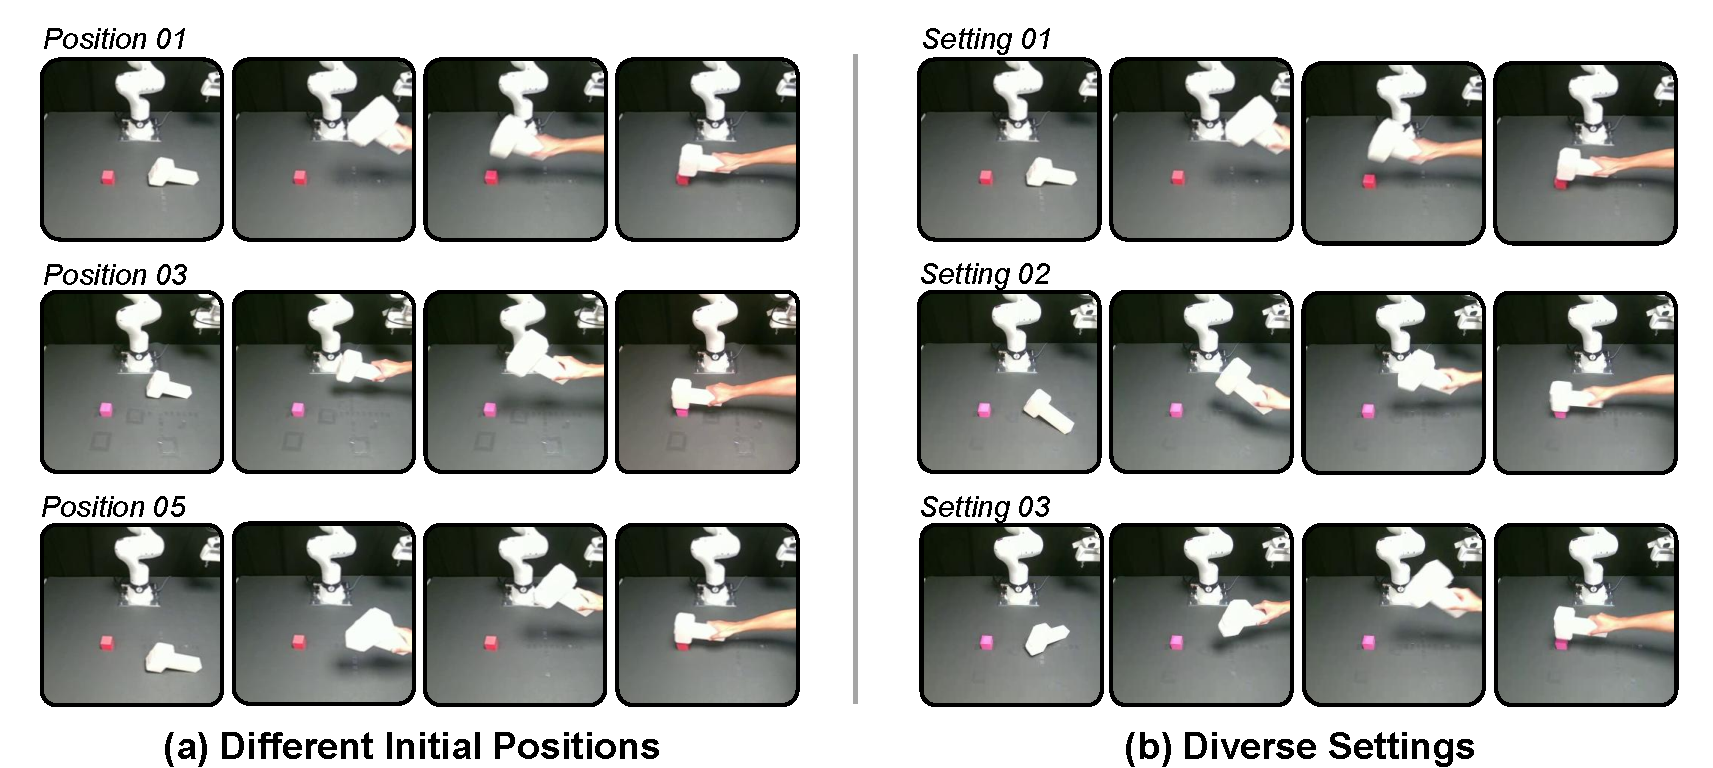
\includegraphics[width=1.0\linewidth]{figures/human-video-prompt.pdf}
    \caption{\textbf{Human Video Prompt Samples.}
    (a) Samples from different initial positions. (b) Samples from different settings.}

    \label{fig:human-video-prompts}
\end{figure}

\textbf{Affordance Images.}~~ 
We manually annotate the grasp point and hitting region for each tool, producing 10 affordance images in total. When evaluating functional intermediate representations in Sec.~\ref{sec:Functional Intermediate Representations Selection}, we use the affordance image of the corresponding tool as an additional condition for the grounded execution policy $\pi_{\mathrm{sys1}}$. Since this representation is time-invariant, the same image feature is shared across all time steps of a trajectory.





\textbf{Human Video Prompts.}~~
As shown in Fig.~\ref{fig:human-video-prompts}, we collect human video prompts for all 7 tools. Following the simulation benchmark, each tool has 3 settings. For each setting, we define 5 initial positions and collect 5 videos per position, resulting in 525 human tool-use videos in total. When evaluating functional intermediate representations, we use the video prompt corresponding to the same tool, setting, and sample from Position 01 as an additional condition for the grounded execution policy. These videos provide visual demonstrations of how humans accomplish the same hitting function with different tools. We further validate that human video data can serve as effective action-free pretraining data for functional reasoning in Sec.~\ref{sec:scalability-human-video}.


\textbf{Functional Videos and Object Masks.}~~
For each simulation demonstration, we use the corresponding ground-truth functional execution video as a temporally varying condition.
To construct object masks, we remove the background from each frame while retaining the tool and target object, thereby preserving object-centric geometry and motion while suppressing background appearance.
Both representations are temporally aligned with the robot trajectory and used as sequential conditions for $\pi_{\mathrm{sys1}}$.
With 10 tools, 3 settings, and 30 randomized initial configurations per setting, we obtain 900 functional-video sequences and 900 object-mask sequences in total.

\textbf{Keypoint Trajectories.}~~
We adopt 2D keypoint trajectories as the final functional intermediate representation and extract them for both simulation and real-world data. In simulation, the hitting and target points are directly obtained from the simulator. Given the initial hitting point on the tool, we use SAM2~\citep{ravi2025sam} to segment the corresponding tool mask and sample $N=5$ additional tool keypoints with Farthest Point Sampling (FPS), ensuring spatial coverage of the tool geometry. We then track these sampled tool keypoints with CoTracker~\citep{karaev2024cotracker} to obtain their 2D trajectories. Our simulation benchmark contains 10 tools with 3 settings each. For each setting, we randomly initialize 30 hitting and target positions, resulting in 900 simulation samples.
For real-world data, we manually annotate the target and hitting points for each sample and obtain five additional tool keypoints using the same SAM2- and FPS-based procedure. Unlike simulation, where the hitting and target trajectories are available from the simulator, all 7 real-world keypoints are tracked by CoTracker. The real-world benchmark contains 7 tools, each with 2 hitting patterns
and 1 initial position. We collect 20 samples for each initial position, resulting in 280 real-world samples. 
% These trajectories are used as action-free supervision, while robot action labels from the evaluation tools are not used to train the execution policy.



\subsection{MPPI-based Demonstration Generation}
\label{app:mppi_annotation}

% In the simulation benchmark, the action-labeled demonstrations are automatically generated rather than collected through teleoperation. We use a Model Predictive Path Integral (MPPI) planner with a four-stage rollout procedure, whose main reward terms are summarized in Tab.~\ref{tab:mppi_rewards}. The stages sequentially encourage the robot to lift the tool, move it toward the target, align the tool-specific hitting point with the target, and execute the final downward strike.
In the simulation benchmark, the action-labeled demonstrations are automatically generated rather than collected through teleoperation.
We use a Model Predictive Path Integral (MPPI) planner with function-specific objectives.
Taking the hitting function as an example, we adopt a four-stage rollout procedure, whose detailed reward terms are summarized in Tab.~\ref{tab:mppi_rewards}.
The stages sequentially encourage the robot to lift the tool, move it toward the target, align the tool-specific hitting point with the target, and execute the final downward strike.

Besides the translational commands optimized by MPPI, we specify a target rotational pose at the end of each stage and generate the corresponding rotational commands through servo control. This helps the tool maintain an appropriate orientation during lifting, alignment, and hitting. Together, the stage-specific MPPI rewards and rotational servo control enable reliable automatic demonstration generation in simulation.


\begin{table}[p]
\centering
\caption{\textbf{Main Reward Terms for MPPI-based Demonstration Generation.}
Here, $d_x$, $d_y$, and $d_{xy}$ denote the distances between the hitting point and the target along the $x$ axis, the $y$ axis, and the $xy$ plane, respectively, while $\Delta d_x$, $\Delta d_y$, and $\Delta d_{xy}$ denote their step-wise reductions.
For the vertical direction, $z_{\mathrm{lift}}$ denotes the tool lifting height from its initial height, $z_1$ denotes the target lifting threshold in Stage~1, $\Delta z_{\mathrm{lift}}$ denotes the step-wise lifting progress, and $e_z$ denotes the error between the current tool height and the target hovering height.
$\Delta z_{\mathrm{head}}$ denotes the vertical displacement of the hitting point between consecutive steps, so $-\Delta z_{\mathrm{head}}$ measures downward motion.
The terms $r_\ast$ reward the current state for satisfying the stage-specific objective, while $r_{\ast\_\mathrm{prog}}$ rewards step-wise progress toward that objective.}

\label{tab:mppi_rewards}
\resizebox{\linewidth}{!}{
\begin{tabular}{lp{0.30\linewidth}p{0.50\linewidth}}
\toprule
Stage & Objective & Main Reward Terms \\
\midrule
Stage 1 
& Lift the tool and align it with the target along the $x$ and $y$ axes.
& 
$
\begin{aligned}
r_{\mathrm{lift}} &= 18.0\min(z_{\mathrm{lift}}, z_1), \\
r_{\mathrm{lift\_prog}} &= 100.0\min(\Delta z_{\mathrm{lift}}, 0.02), \\
r_x &= 22.0\exp(-18.0 d_x), \\
r_{x\_\mathrm{prog}} &= 120.0\min(\Delta d_x, 0.02), \\
r_y &= 8.0\exp(-8.0 d_y), \\
r_{y\_\mathrm{prog}} &= 35.0\min(\Delta d_y, 0.02).
\end{aligned}
$
\\
\midrule
Stage 2 
& Move the tool toward the target while maintaining a suitable hovering height. 
& 
$
\begin{aligned}
r_{xy} &= 14.0\exp(-10.0 d_{xy}), \\
r_x &= 12.0\exp(-18.0 d_x), \\
r_y &= 8.0\exp(-10.0 d_y), \\
r_z &= 7.0\exp(-18.0 e_z), \\
r_{xy\_\mathrm{prog}} &= 95.0\min(\Delta d_{xy}, 0.02), \\
r_{x\_\mathrm{prog}} &= 80.0\min(\Delta d_x, 0.02), \\
r_{y\_\mathrm{prog}} &= 40.0\min(\Delta d_y, 0.02).
\end{aligned}
$
\\
\midrule
Stage 3 
& Finely align the tool-specific hitting point above the target. 
& 
$
\begin{aligned}
r_{xy} &= 14.0\exp(-14.0 d_{xy}), \\
r_x &= 14.0\exp(-24.0 d_x), \\
r_y &= 10.0\exp(-18.0 d_y), \\
r_{xy\_\mathrm{prog}} &= 145.0\min(\Delta d_{xy}, 0.018), \\
r_{x\_\mathrm{prog}} &= 135.0\min(\Delta d_x, 0.018), \\
r_{y\_\mathrm{prog}} &= 110.0\min(\Delta d_y, 0.018), \\
r_z &= 7.0\exp(-18.0 e_z).
\end{aligned}
$
\\
\midrule
Stage 4 
& Keep the hitting point close to the target and execute the downward strike. 
& 
$
\begin{aligned}
r_{xy} &= 12.0\exp(-16.0 d_{xy}), \\
r_x &= 14.0\exp(-28.0 d_x), \\
r_y &= 10.0\exp(-18.0 d_y), \\
r_{xy\_\mathrm{prog}} &= 120.0\min(\Delta d_{xy}, 0.015), \\
r_{x\_\mathrm{prog}} &= 100.0\min(\Delta d_x, 0.015), \\
r_{y\_\mathrm{prog}} &= 80.0\min(\Delta d_y, 0.015), \\
r_{\mathrm{hit}} &= 150.0\min(-\Delta z_{\mathrm{head}}, 0.05),
\end{aligned}
$
\\
\midrule
Contact / Success 
& Encourage valid downward contact with the target.
& 
$
\begin{aligned}
r_{\mathrm{contact}} &= 150.0 \ \text{if valid downward contact}.
\end{aligned}
$
\\
\bottomrule
\end{tabular}
}
\end{table}
\FloatBarrier

\subsection{Training and Implementation Details}
\label{app:implementation_details}

All models are trained on NVIDIA RTX 6000 Pro GPUs. For all methods, we use an action chunk size of 8, a history horizon of 8, and a batch size of 64. We build the simulation benchmark on Robomimic and conduct real-world experiments on a Franka robot platform.

For baseline methods, we train each policy for 120,000 steps using the corresponding action-labeled data. For \algoname{}, we follow the two-stage training procedure described in Sec.~\ref{sec:FORGE}. 
%We first pretrain the keypoint motion predictor $\pi_{\mathrm{sys2}}$ on action-free data from all tools for 240,000 steps.
We first pretrain the keypoint motion predictor $\pi_{\mathrm{sys2}}$ on independently collected action-free data for 240,000 steps.
We then freeze the pretrained predictor and fine-tune the grounded execution policy $\pi_{\mathrm{sys1}}$ on the same action-labeled data used by the baselines for 120,000 steps.


\section{Additional Experimental Results}
\label{app:additional_experimental_results}

This section provides additional qualitative comparisons across hitting, sweeping, and hooking in both the real world and simulation. These results complement the quantitative evaluations in the main paper by illustrating representative failure modes of the baselines and how \algoname{} addresses them through function-aware keypoint motion planning.

\begin{figure}[!htbp]
    \centering
    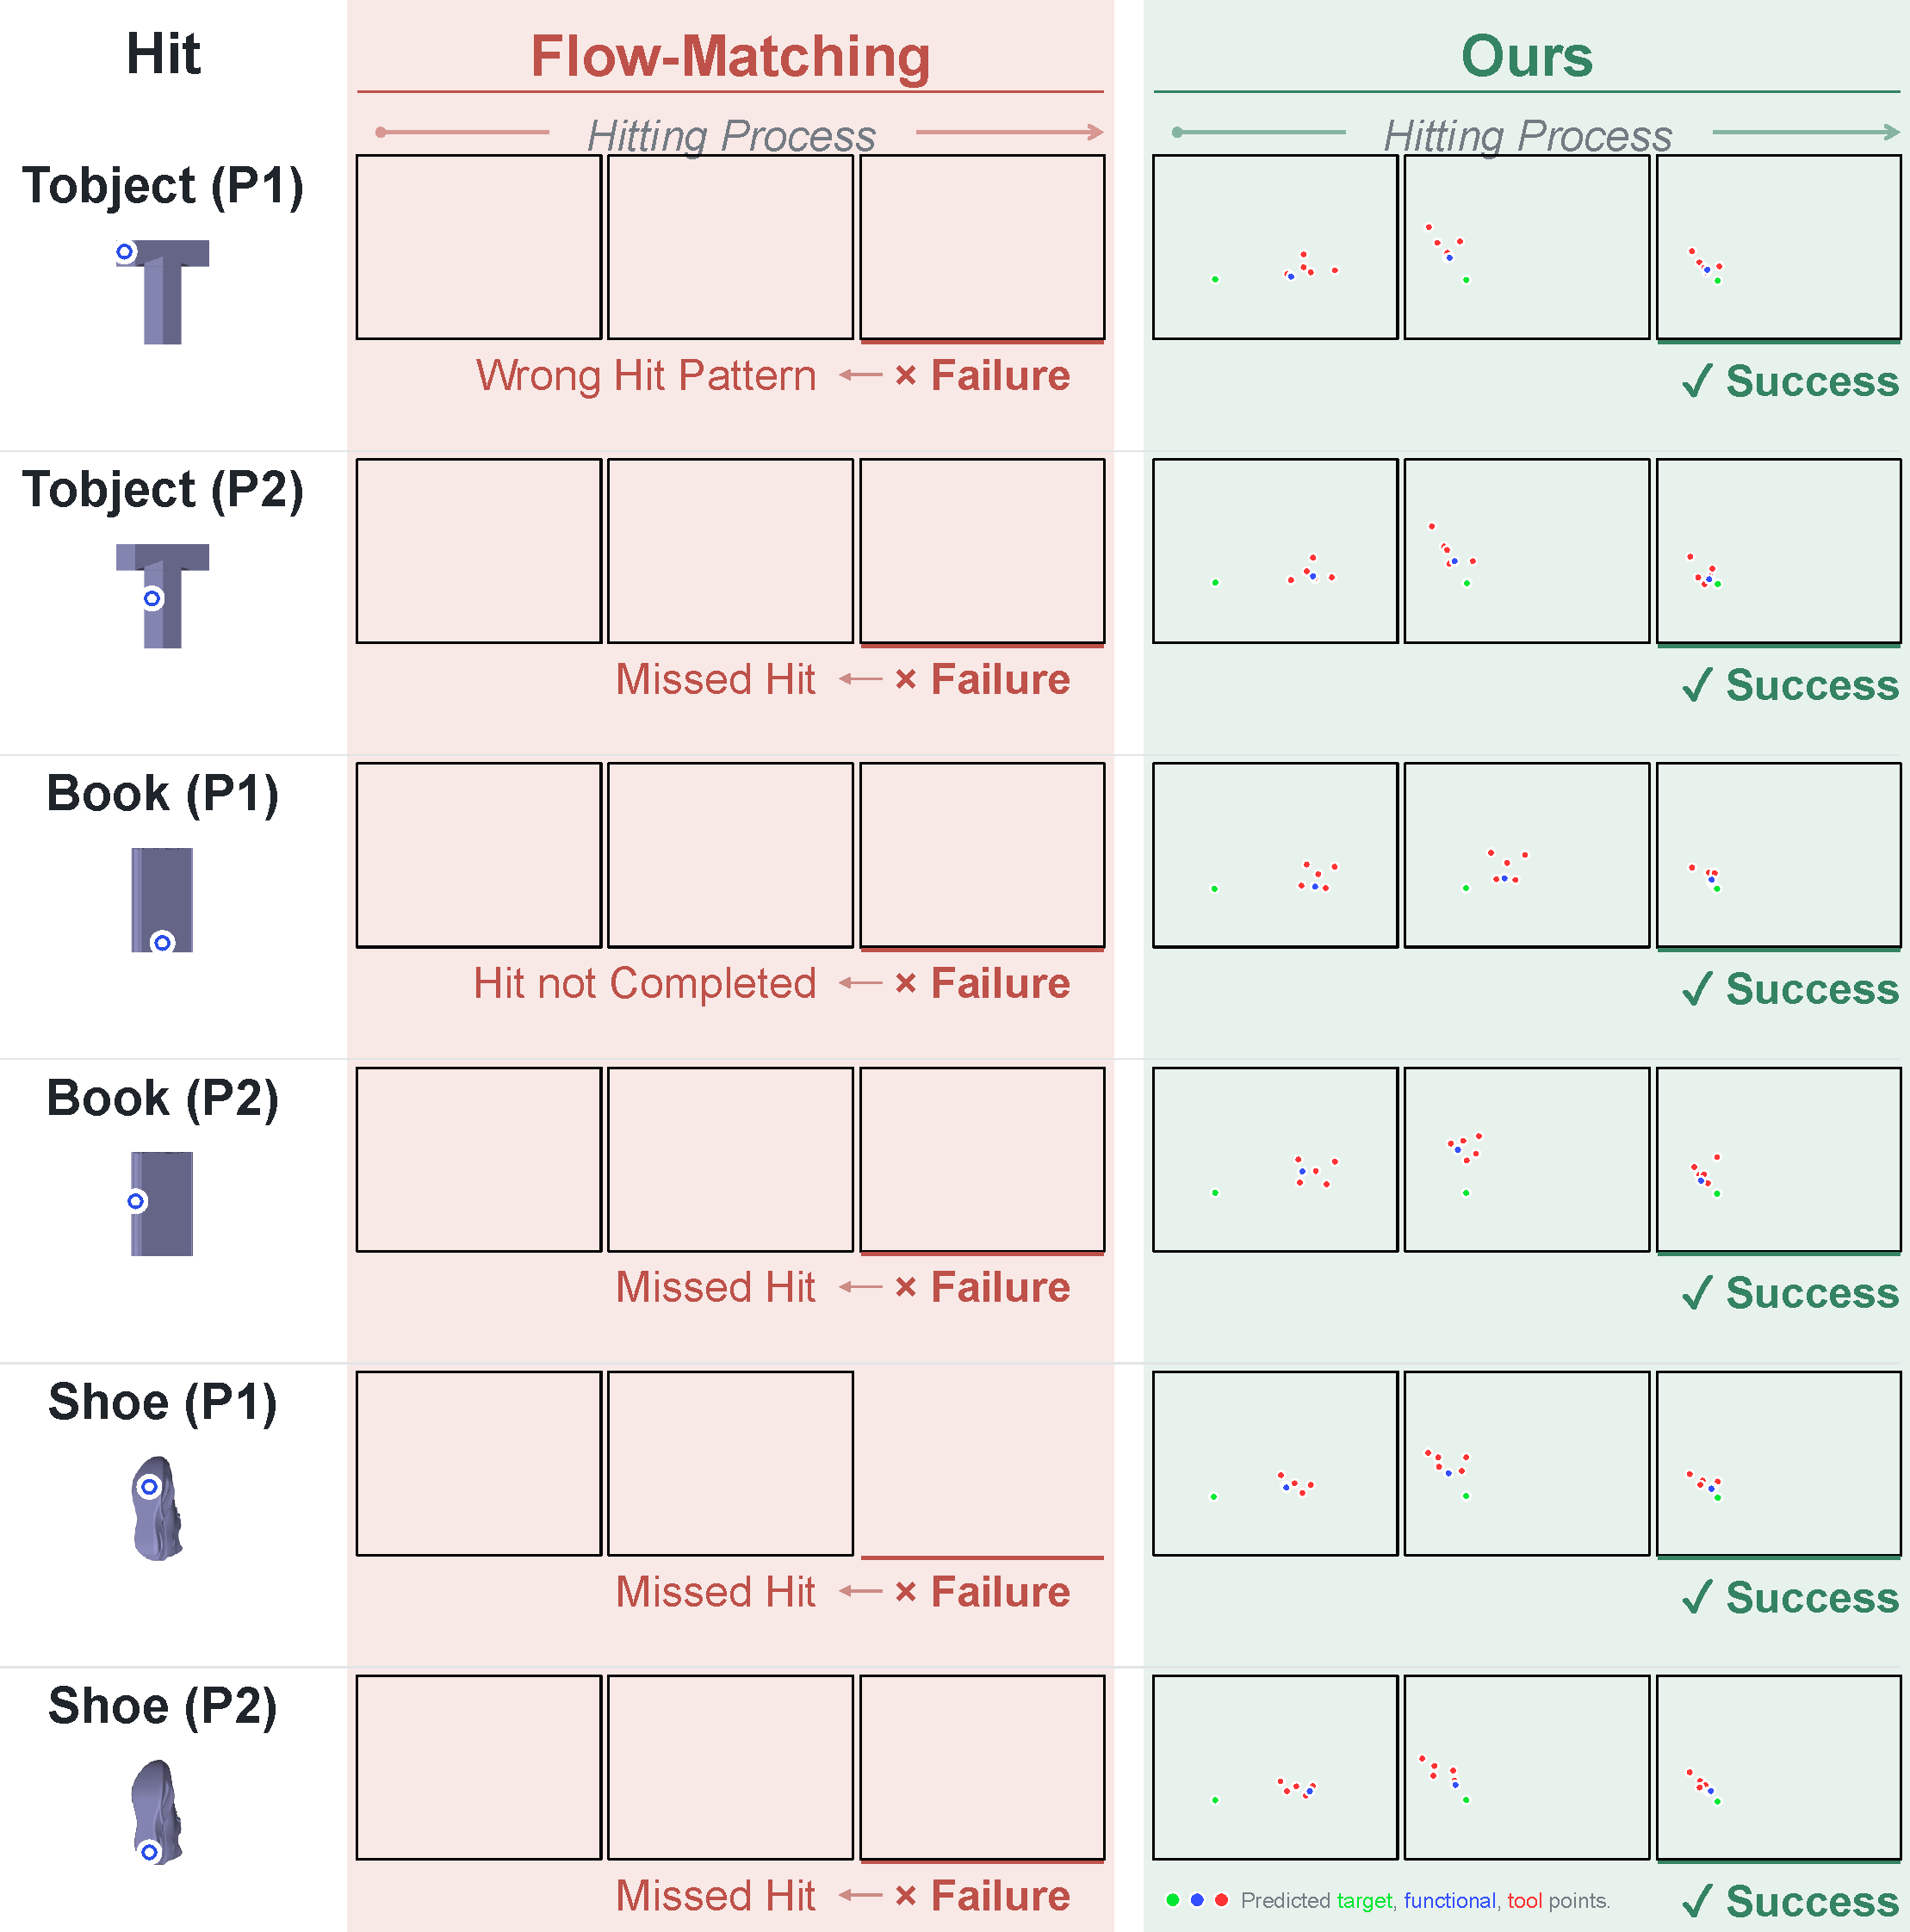
\includegraphics[width=0.82\linewidth]{figures/app-hitting-real.pdf}
    \caption{\textbf{Real-World Qualitative Results for Hitting.} Failures of the FM baseline and successful demos of \algoname{} on unseen tools across hitting patterns. The blue point indicates the reference hitting point for each pattern.}
    \label{fig:app-real-hitting}
\end{figure}

\begin{figure}[!htbp]
    \centering
    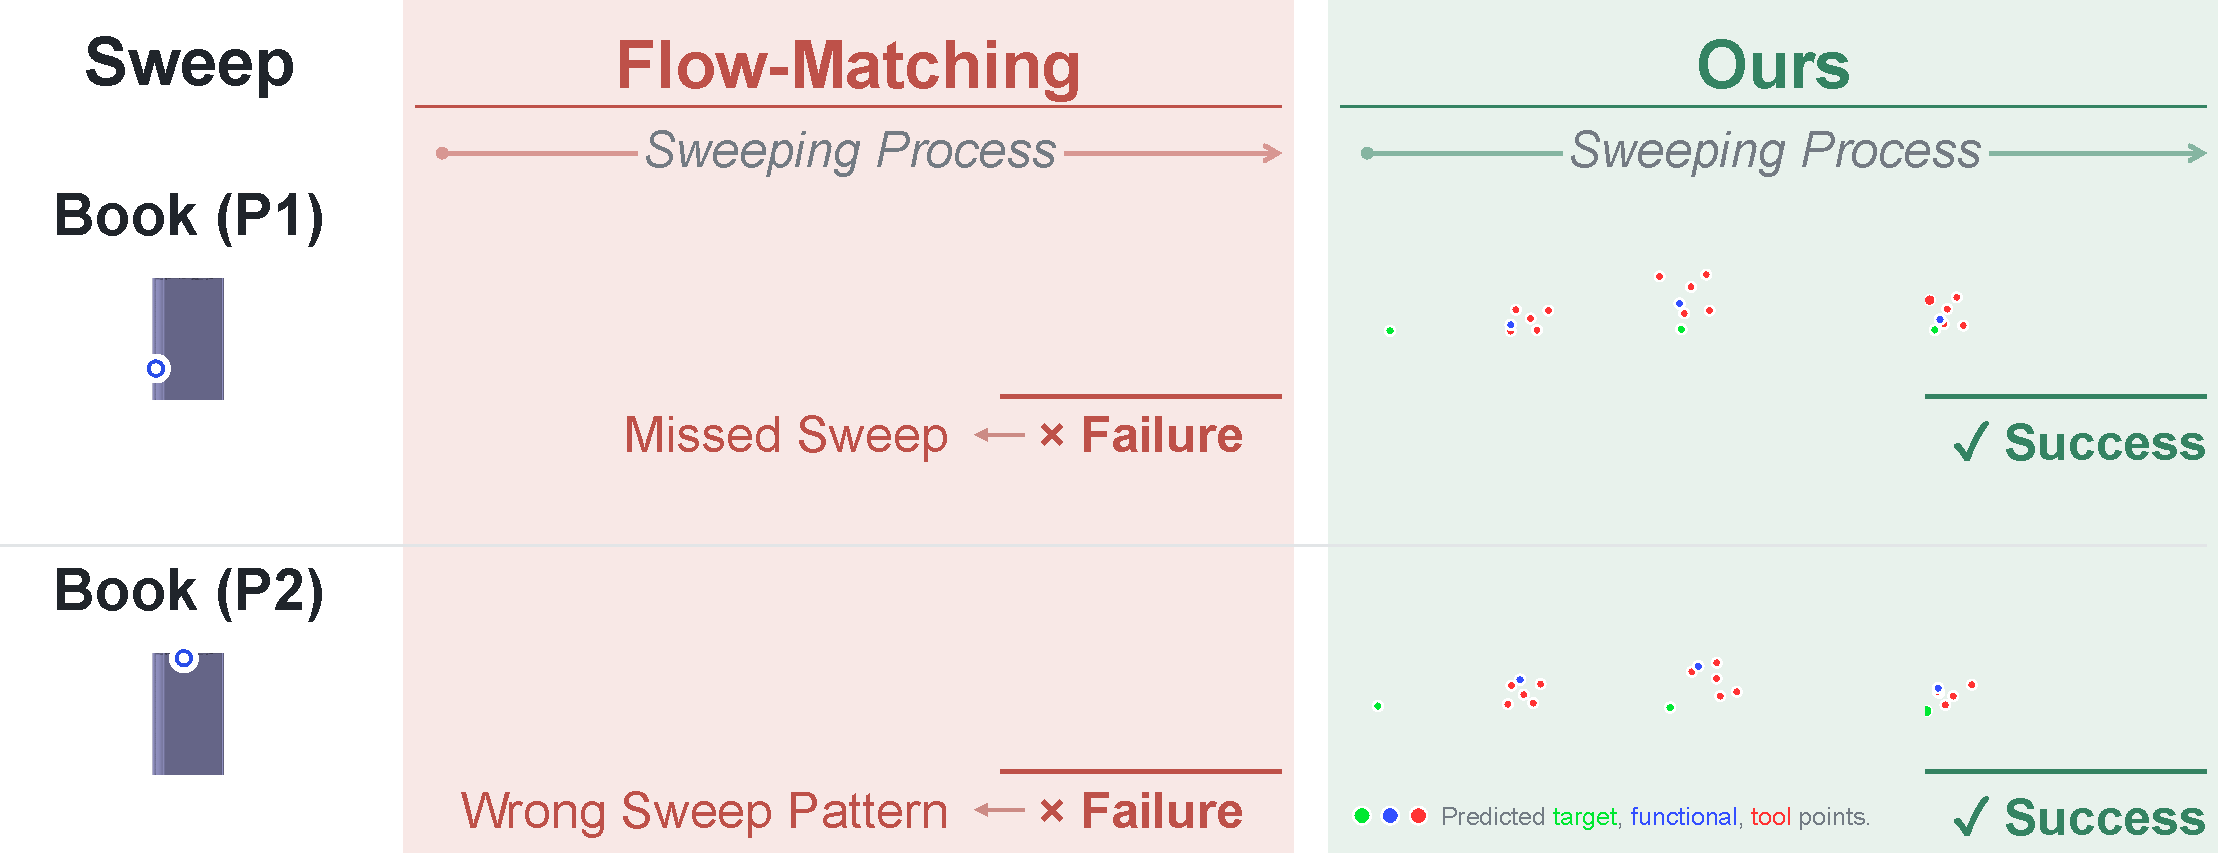
\includegraphics[width=0.82\linewidth]{figures/app-sweeping-real.pdf}
    \caption{\textbf{Real-World Qualitative Results for Sweeping.} Failures of the FM baseline and successful demos of \algoname{} on unseen tools across sweeping patterns. The blue point indicates the reference sweeping point for each pattern.}
    \label{fig:app-real-sweeping}
\end{figure}

\begin{figure}[!htbp]
    \centering
    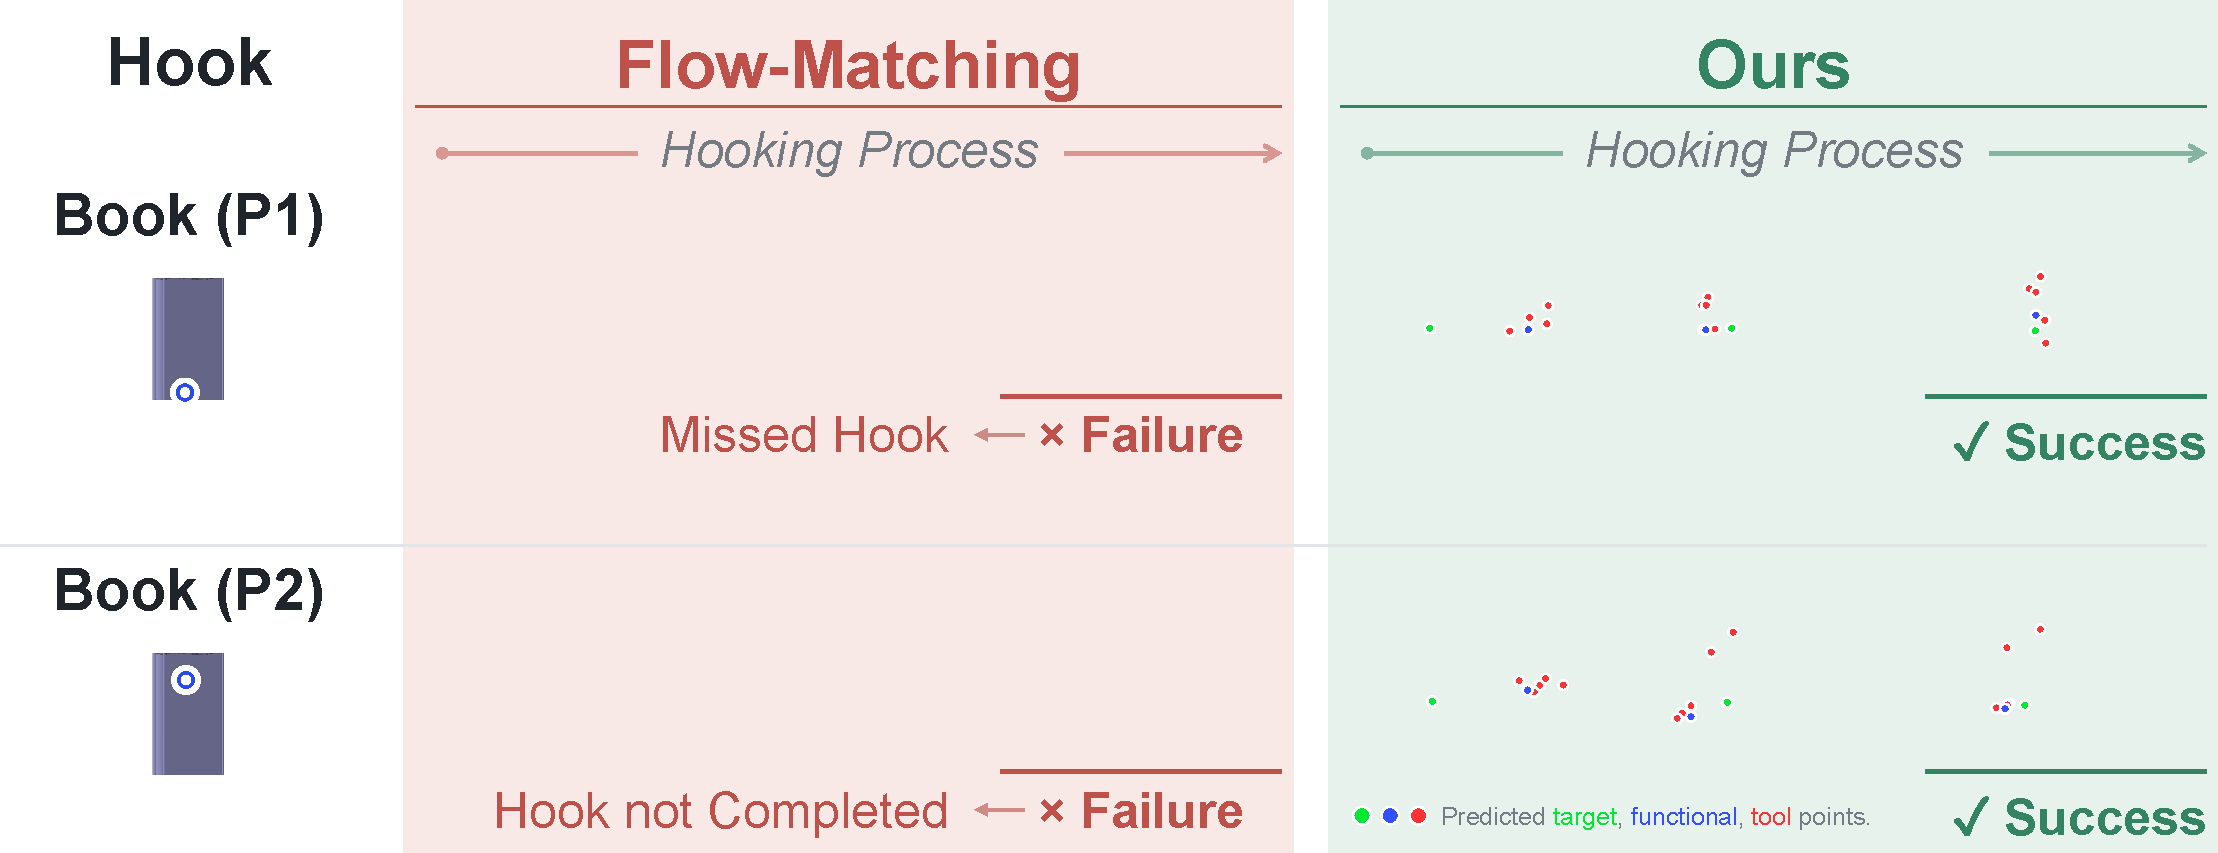
\includegraphics[width=0.82\linewidth]{figures/app-hooking-real.pdf}
    \caption{\textbf{Real-World Qualitative Results for Hooking.} Failures of the FM baseline and successful demos of \algoname{} on unseen tools across hooking patterns. The blue point indicates the reference hooking point for each pattern.}
     \label{fig:app-real-hooking}
\end{figure}


\FloatBarrier
\subsection{More Qualitative Results in the Real World}
\label{app:more_qualitative_results_real}

Figs.~\ref{fig:app-real-hitting}--\ref{fig:app-real-hooking} provide additional real-world comparisons between the FM baseline and \algoname{} across hitting, sweeping, and hooking on unseen tools and different functional patterns.
Across the three functions, FM exhibits representative failure modes including missed or incomplete interactions and incorrect functional motion patterns, showing that an end-to-end policy struggles to adapt both the functional region and the required motion to novel tool geometries.
By contrast, \algoname{} uses predicted keypoint-based functional plans to guide functional-region alignment and motion execution, leading to successful interactions across the shown hitting, sweeping, and hooking cases.
These results further demonstrate the benefit of an explicit function-aware intermediate representation for functional generalization.



\begin{figure}[!htbp]
    \centering
    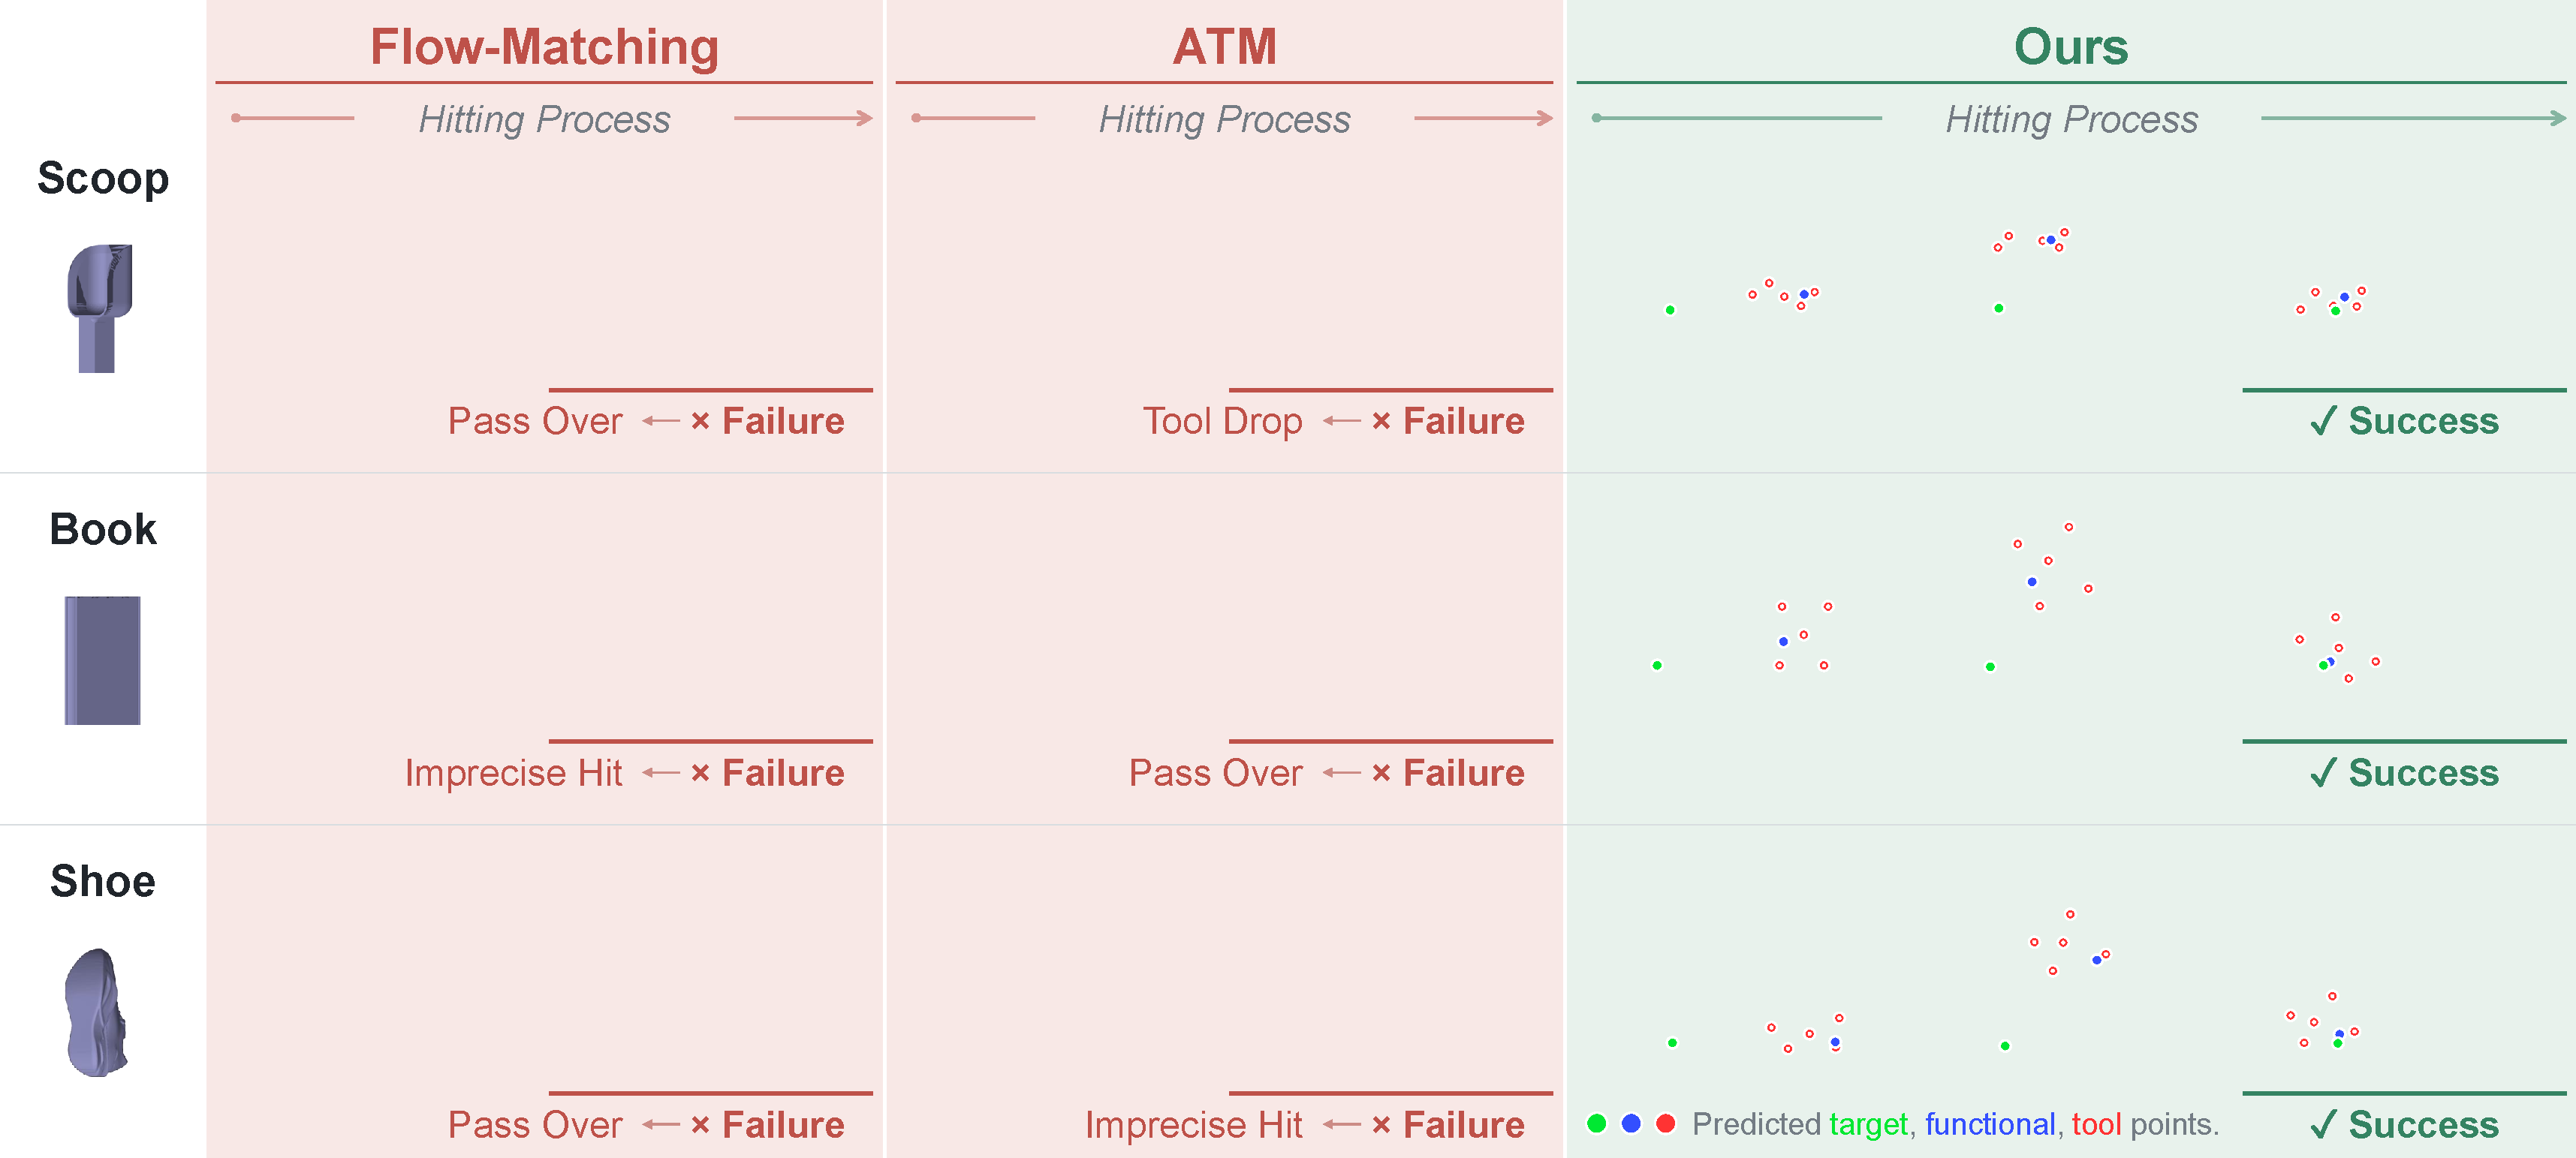
\includegraphics[width=0.82\linewidth]{figures/app-hitting-sim.pdf}
    \caption{\textbf{Simulation Qualitative Results for Hitting.} Failures of FM and ATM and successful rollouts of \algoname{} on unseen tools.}
    \label{fig:app-hitting-sim}
\end{figure}

\begin{figure}[!htbp]
    \centering
    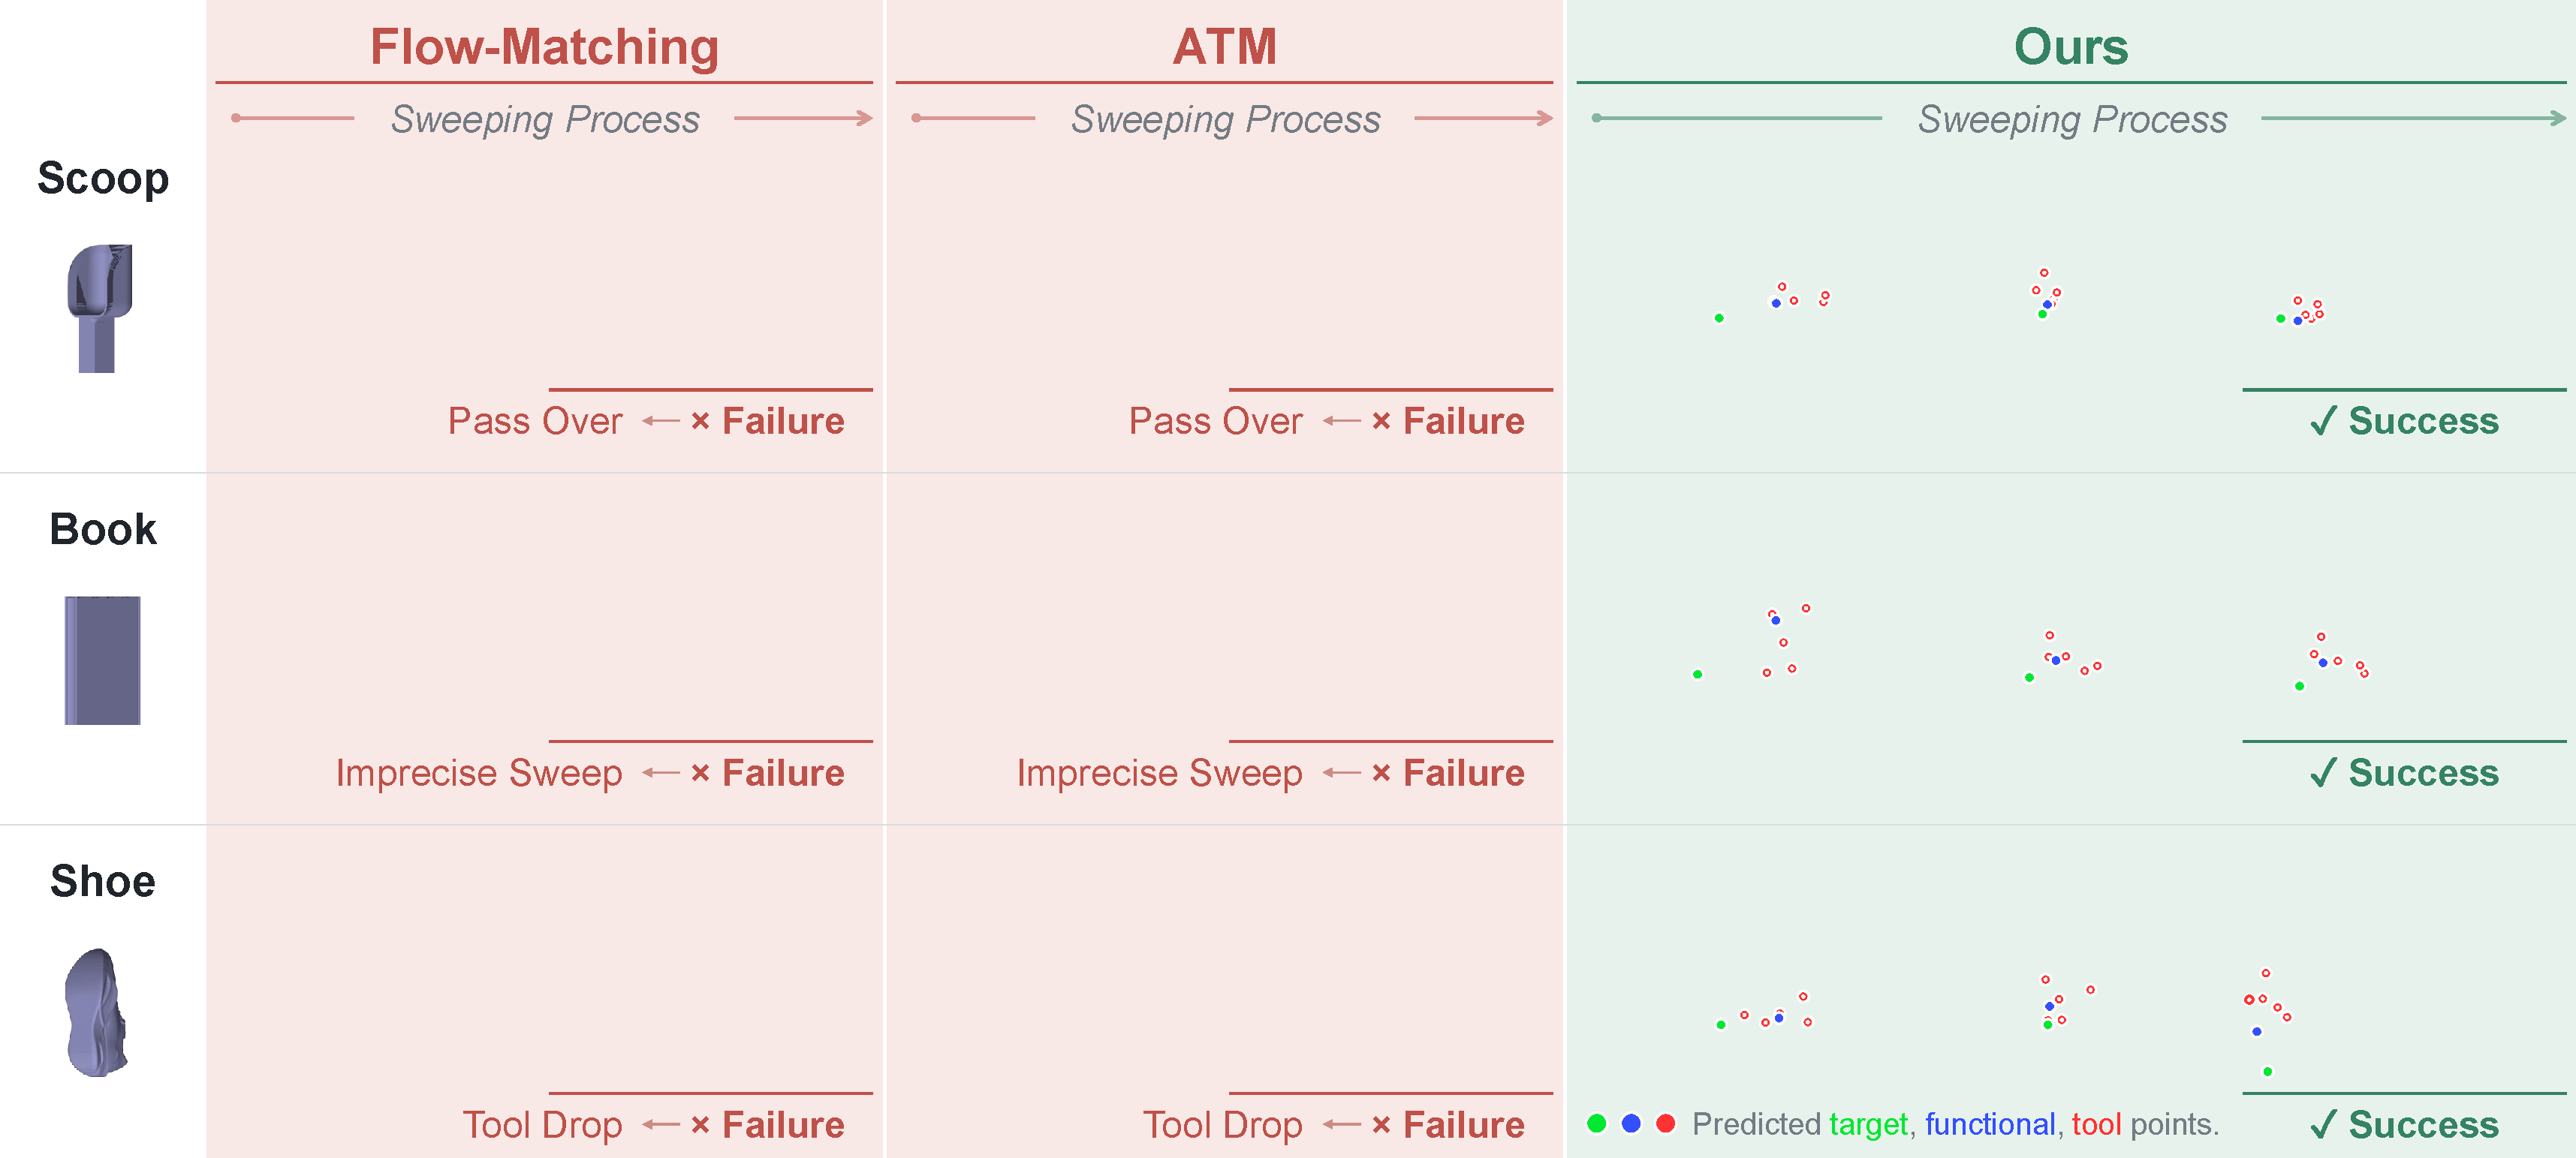
\includegraphics[width=0.82\linewidth]{figures/app-sweeping-sim.pdf}
    \caption{\textbf{Simulation Qualitative Results for Sweeping.} Failures of FM and ATM and successful rollouts of \algoname{} on unseen tools.}
    \label{fig:app-sweeping-sim}
\end{figure}

\begin{figure}[!htbp]
    \centering
    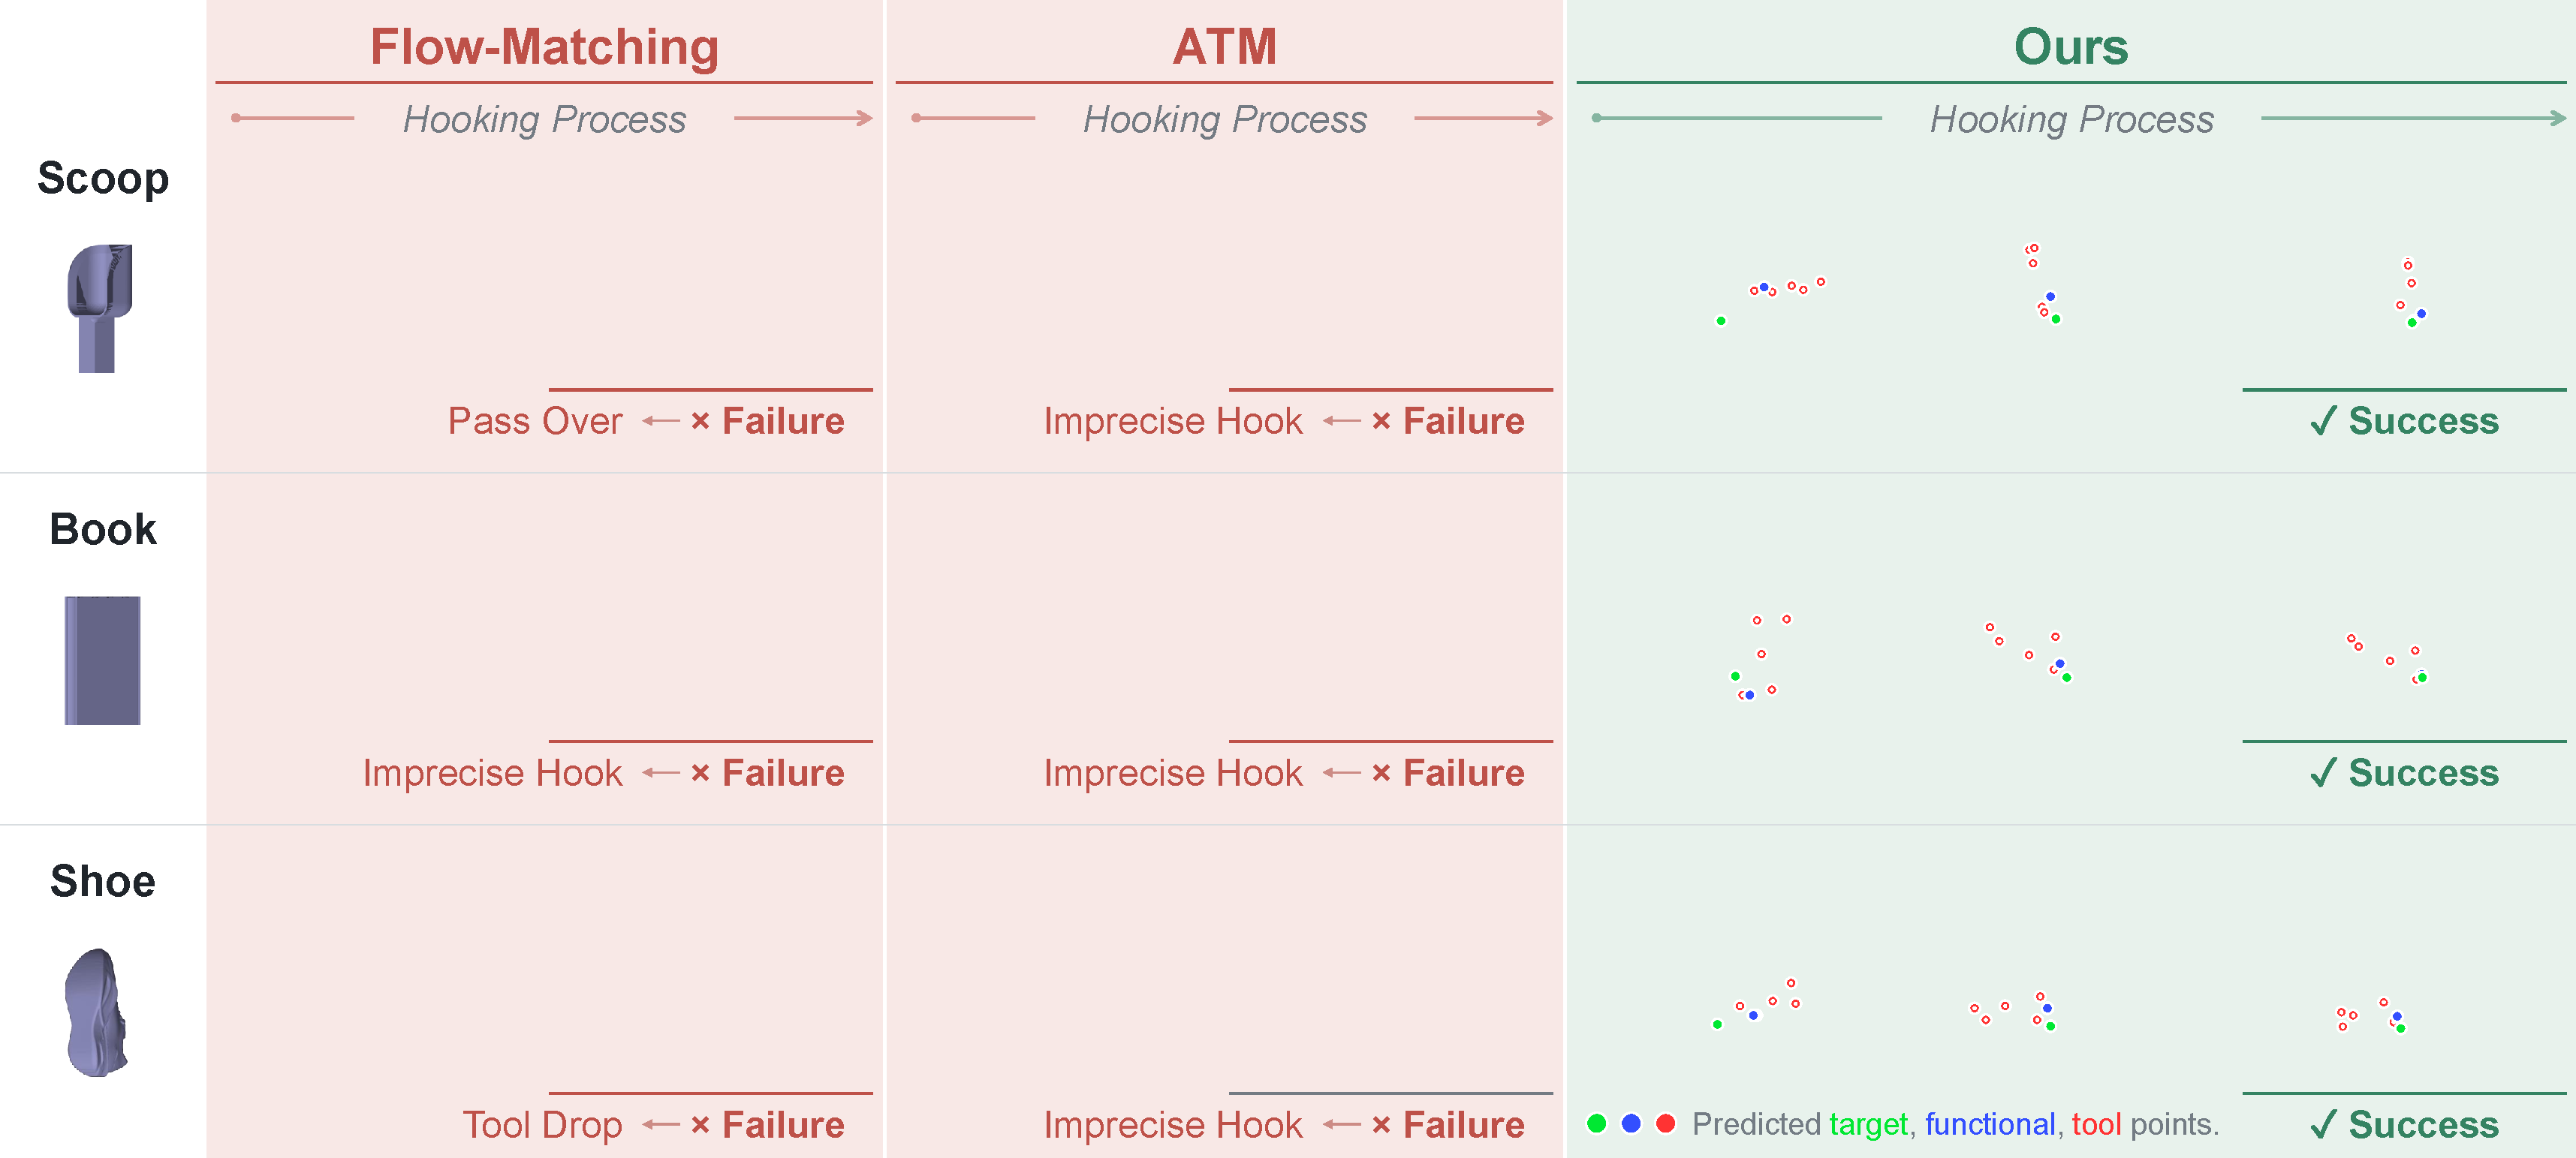
\includegraphics[width=0.82\linewidth]{figures/app-hooking-sim.pdf}
    \caption{\textbf{Simulation Qualitative Results for Hooking.} Failures of FM and ATM and successful rollouts of \algoname{} on unseen tools.}
    \label{fig:app-hooking-sim}
\end{figure}


\FloatBarrier
\subsection{More Qualitative Results in Simulation}
\label{app:more_qualitative_results_sim}

Figs.~\ref{fig:app-hitting-sim}--\ref{fig:app-hooking-sim} provide additional simulation comparisons among FM, ATM, and \algoname{} across hitting, sweeping, and hooking on unseen tools.
FM exhibits representative failures such as passing over the target, imprecise interactions, and tool dropping.
Although ATM also conditions on keypoint trajectories, its generic trajectories do not explicitly encode function-specific motion intent and can therefore exhibit similar failures.
In contrast, \algoname{} predicts function-aware keypoint trajectories that explicitly guide how the functional region should move toward and interact with the target, enabling more reliable execution across the three functions.


Please refer to our supplementary videos for complete rollouts of both simulation and real-world experiments.